% !TeX program = lualatex
% ^ Compile with LuaLaTeX (or XeLaTeX). On Overleaf: Menu -> Compiler -> LuaLaTeX.
%   Under pdfLaTeX the theme falls back to Latin Modern Sans (see beamerthemegemini.sty).

\documentclass[final]{beamer}

% ====================
% Packages
% ====================

\usepackage[T1]{fontenc}
\usepackage{lmodern}
\usepackage[size=custom,width=120,height=90,scale=0.92]{beamerposter}
\usetheme{gemini}
\usecolortheme{cam}
% ---- Times for everything ----------------------------------------------------
% TeX Gyre Termes is the free Times clone bundled with TeX Live, so the local preview
% and Overleaf render with the identical font file (Times New Roman proper is a
% Microsoft font that TeX Live does not ship). The theme sets sans-serif Lato and
% Raleway; this replaces both, and sets the math font to match.
\ifPDFTeX
  \usepackage{newtxtext,newtxmath}
  \renewcommand{\familydefault}{\rmdefault}
  \renewcommand{\Raleway}{\rmfamily}
  \renewcommand{\Lato}{\rmfamily}
\else
  \usepackage{unicode-math}
  \setmainfont{TeX Gyre Termes}
  \setsansfont{TeX Gyre Termes}
  \renewfontfamily\Raleway{TeX Gyre Termes}
  \renewfontfamily\Lato{TeX Gyre Termes}
  \setmathfont{TeX Gyre Termes Math}
\fi
\usepackage{graphicx}
\usepackage{booktabs}
\usepackage{tikz}
\usetikzlibrary{svg.path}
\usepackage{pgfplots}
\pgfplotsset{compat=1.14}
\usepackage{anyfontsize}
\usepackage{comment}
\usepackage{xcolor}

% The theme draws the header with 'headline title' / 'headline author', so those are the
% fonts that matter. Sizes are absolute: the poster is fixed at 120 x 90 cm.
\setbeamerfont{headline title}{size={\fontsize{62}{73}},series=\bfseries}
\setbeamerfont{headline author}{size={\fontsize{38}{46}}}
\setbeamerfont{headline institute}{size={\fontsize{30}{36}}}
\setbeamerfont{block title}{size={\fontsize{44}{54}}}
\setbeamerfont{block body}{size=\large}
\setbeamerfont{caption}{size=\normalsize}
% Beamer sets \raggedright INSIDE each list, after the body-begin template, so a
% template hook is overwritten. \beamer@firstlineitemizeunskip runs right after it
% in itemize, enumerate and description, so justify there instead.
\makeatletter
\let\beamer@origfirstlineunskip\beamer@firstlineitemizeunskip
\def\beamer@firstlineitemizeunskip{\justifying\beamer@origfirstlineunskip}
\makeatother

\usepackage[skip=12pt]{caption}   % 2pt is absolute and does not scale: the rule hit the caption
\usepackage{microtype}            % protrusion + expansion: fewer bad line breaks
\usepackage[backend=biber]{biblatex}
\addbibresource{ref.bib}

% --- Official blues ---
\definecolor{PrimaryBlue}{RGB}{29,79,145}
\definecolor{SecondaryBlue1}{RGB}{0,48,135}
\definecolor{SecondaryBlue2}{RGB}{0,119,200}
\definecolor{SecondaryBlue3}{RGB}{108,172,228}

% --- Neutral ---
\definecolor{Neutral1}{RGB}{34,34,34}
\definecolor{Neutral2}{RGB}{83,86,90}
\definecolor{Neutral3}{RGB}{208,208,206}
\definecolor{Neutral4}{RGB}{240,240,240}

% --- Accent ---
\definecolor{Accent1}{RGB}{199,80,0}
\definecolor{Transactional1}{RGB}{142,75,53}
\definecolor{Transactional2}{RGB}{220,42,42}
\definecolor{DodgerBlue}{RGB}{0,162,255}

% ====================
% Lengths
% ====================

\newlength{\sepwidth}
\newlength{\colwidth}
\setlength{\sepwidth}{0.025\paperwidth}
\setlength{\colwidth}{0.3\paperwidth}
% Every paragraph's last line must be at least a quarter of a column (~3-4 words),
% so no line ends with a single stranded word. Measured against the COLUMN: in
% beamerposter \textwidth is the whole poster, which would constrain nothing.
\setlength{\parfillskip}{0pt plus 0.75\colwidth}
% The theme calls \justifying (ragged2e) in every block body, and \justifying resets
% \parfillskip to \JustifyingParfillskip. Set that too, or the rule never applies.
\setlength{\JustifyingParfillskip}{0pt plus 0.75\colwidth}

\newcommand{\separatorcolumn}{\begin{column}{\sepwidth}\end{column}}
\newcommand{\email}[1]{\def\insertemail{#1}}
\newsavebox{\laidlawbox}
% Laidlaw Foundation logo: official white SVG (laidlawfoundation.com), converted to
% native TikZ vector paths. #1 = printed height. yscale=-1 turns SVG's downward y-axis
% upright; \resizebox fixes the height exactly regardless of internal units.
\newcommand{\laidlawlogo}[1]{\resizebox{!}{#1}{%
  \begin{tikzpicture}[yscale=-1]
    \fill[white] svg {M 26.4 19.6 L 37.5 38.8 L 1.1 38.8 L 3.7 34.2 L 29.5 34.2 L 23.8 24.2 L 26.4 19.6 Z};
    \fill[white] svg {M 26.8 32.6 L 4.6 32.6 L 22.8 1.1 L 25.5 5.7 L 12.7 28 L 24.1 28 L 26.8 32.6 Z};
    \fill[white] svg {M 15.4 26.4 L 26.4 7.3 L 44.6 38.8 L 39.3 38.8 L 26.4 16.5 L 20.7 26.4 L 15.4 26.4 Z};
    \fill[white] svg {M 49 28.3 V 13 h 3.7 v 12.1 h 6.1 v 3.2 H 49 z};
    \fill[white] svg {M 70.5 28.3 l -1.2 -3.2 h -5 l -1.2 3.2 h -3.5 l 6 -15.4 h 2.6 l 6 15.4 H 70.5 z M 67.3 19.3 c -0.2 -0.4 -0.3 -1 -0.5 -1.6 h 0 c -0.1 0.6 -0.3 1.1 -0.5 1.6 l -1.1 3.1 h 3.2 L 67.3 19.3 z};
    \fill[white] svg {M 76 28.3 V 13 h 3.7 v 15.3 H 76 z};
    \fill[white] svg {M 87.8 28.3 h -5.2 V 13 h 5.2 c 4.4 0 8.2 2.9 8.2 7.7 S 92.2 28.3 87.8 28.3 z M 87.3 16.2 h -1.2 v 8.9 h 1.2 c 2.7 0 4.9 -1.5 4.9 -4.5 C 92.2 17.7 90 16.2 87.3 16.2 z};
    \fill[white] svg {M 98.1 28.3 V 13 h 3.7 v 12.1 h 6.1 v 3.2 H 98.1 z};
    \fill[white] svg {M 119.6 28.3 l -1.2 -3.2 h -5 l -1.2 3.2 h -3.5 l 6 -15.4 h 2.6 l 6 15.4 H 119.6 z M 116.4 19.3 c -0.2 -0.4 -0.3 -1 -0.5 -1.6 h 0 c -0.1 0.6 -0.3 1.1 -0.5 1.6 l -1.1 3.1 h 3.2 L 116.4 19.3 z};
    \fill[white] svg {M 138.8 28.4 h -2.4 l -2.2 -6.8 c -0.3 -1 -0.7 -2.1 -1 -3.4 h 0 c -0.3 1.3 -0.7 2.4 -1 3.4 l -2.2 6.8 h -2.4 L 122.4 13 h 3.6 l 2 6.2 c 0.3 0.9 0.6 1.9 0.8 3.1 h 0 c 0.2 -1.2 0.5 -2.1 0.8 -3.1 l 2 -6.2 h 3.2 l 2 6.2 c 0.3 0.8 0.6 2 0.8 3.1 h 0 c 0.2 -1.1 0.5 -2.2 0.8 -3.1 l 2 -6.2 h 3.3 L 138.8 28.4 z};
    \fill[white] svg {M 49.7 33.1 v 2.3 H 52 V 36 h -2.3 v 2.9 H 49 v -6.4 h 3.4 v 0.6 H 49.7 z};
    \fill[white] svg {M 59.5 39 c -1.8 0 -3.3 -1.3 -3.3 -3.3 c 0 -2 1.6 -3.3 3.3 -3.3 c 1.8 0 3.3 1.3 3.3 3.3 C 62.8 37.7 61.3 39 59.5 39 z M 59.5 33 c -1.4 0 -2.7 1.1 -2.7 2.7 s 1.3 2.7 2.7 2.7 c 1.4 0 2.7 -1.1 2.7 -2.7 S 60.9 33 59.5 33 z};
    \fill[white] svg {M 69.6 39 c -1.5 0 -2.5 -0.9 -2.5 -2.3 v -4.2 h 0.7 v 4.1 c 0 1.1 0.7 1.8 1.8 1.8 c 1.1 0 1.8 -0.7 1.8 -1.8 v -4.1 h 0.6 v 4.2 C 72.1 38.1 71.1 39 69.6 39 z};
    \fill[white] svg {M 82.1 39 l -3.1 -3.6 c -0.5 -0.6 -1.1 -1.3 -1.6 -1.8 l 0 0 c 0 0.6 0 1.2 0 1.8 v 3.5 h -0.7 v -6.4 h 0.5 l 3 3.4 c 0.4 0.5 1 1.2 1.4 1.7 l 0 0 c 0 -0.6 0 -1.1 0 -1.7 v -3.4 h 0.7 V 39 H 82.1 z};
    \fill[white] svg {M 88.5 38.9 h -1.7 v -6.4 h 1.7 c 1.9 0 3.5 1.2 3.5 3.2 C 92.1 37.7 90.4 38.9 88.5 38.9 z M 88.4 33.1 h -0.9 v 5.2 h 0.9 c 1.7 0 2.9 -0.9 2.9 -2.6 S 90.1 33.1 88.4 33.1 z};
    \fill[white] svg {M 100.4 38.9 l -0.7 -1.8 H 97 l -0.7 1.8 h -0.7 l 2.6 -6.5 h 0.2 l 2.6 6.5 H 100.4 z M 98.7 34.6 c -0.1 -0.3 -0.2 -0.6 -0.3 -1 h 0 c -0.1 0.3 -0.2 0.7 -0.3 1 l -0.8 2 h 2.2 L 98.7 34.6 z};
    \fill[white] svg {M 106.8 33.1 v 5.8 h -0.7 v -5.8 h -2.2 v -0.6 h 5.1 v 0.6 H 106.8 z};
    \fill[white] svg {M 113.1 38.9 v -6.4 h 0.7 v 6.4 H 113.1 z};
    \fill[white] svg {M 121.6 39 c -1.8 0 -3.3 -1.3 -3.3 -3.3 c 0 -2 1.6 -3.3 3.3 -3.3 c 1.8 0 3.3 1.3 3.3 3.3 C 124.9 37.7 123.3 39 121.6 39 z M 121.6 33 c -1.4 0 -2.7 1.1 -2.7 2.7 s 1.3 2.7 2.7 2.7 c 1.4 0 2.7 -1.1 2.7 -2.7 S 123 33 121.6 33 z};
    \fill[white] svg {M 134.6 39 l -3.1 -3.6 c -0.5 -0.6 -1.1 -1.3 -1.6 -1.8 l 0 0 c 0 0.6 0 1.2 0 1.8 v 3.5 h -0.7 v -6.4 h 0.5 l 3 3.4 c 0.4 0.5 1 1.2 1.4 1.7 l 0 0 c 0 -0.6 0 -1.1 0 -1.7 v -3.4 h 0.7 V 39 H 134.6 z};
  \end{tikzpicture}}}

\newcommand{\callout}[1]{{\fontsize{62}{70}\selectfont\bfseries\color{PrimaryBlue}#1}}
\newcommand{\calloutcap}[1]{\parbox[t]{0.31\linewidth}{\centering\normalsize #1}}

% ====================
% Title
% ====================

\title{Allocation Under Scarce Capacity:\\
Equity-Aware Routing for Urban Food Rescue in New York City}

\author{Skylar Tian \inst{1} \and Faculty Mentor: George Dragomir \inst{1}}

\institute[shortinst]{\inst{1} Columbia University in the City of New York}

% ====================
% Footer
% ====================

\footercontent{
  Laidlaw Undergraduate Research and Leadership Program \hfill
  Research Symposium 2026 $\mid$ Columbia University
  \hfill
  h.tian@columbia.edu
}

% ====================
% Body
% ====================

\begin{document}
\sbox{\laidlawbox}{\laidlawlogo{4.4cm}}
\addtobeamertemplate{headline}{}
{
    \begin{tikzpicture}[remember picture,overlay]
      \node[anchor=west, inner sep=0] at ([xshift=3cm, yshift=-5.6cm]current page.north west)
        {
\includegraphics[height=3.6cm]{logos/Columbia_University_Logo-white.png}};
      \node[anchor=east, inner sep=0] at ([xshift=-3cm, yshift=-5.6cm]current page.north east)
        {\usebox{\laidlawbox}};
    \end{tikzpicture}
    % Barnard logo intentionally omitted (this template shipped with it).
    % QR code intentionally omitted (no public repo yet).
}

\begin{frame}[t]

% ---------------------------------------------------------------- takeaway banner
{\centering\setlength{\fboxsep}{0.45em}%
\colorbox{Neutral4}{\parbox{\dimexpr0.95\paperwidth-2\fboxsep\relax}{\centering
  {\fontsize{46}{56}\selectfont\bfseries\color{PrimaryBlue}%
  Reach $\neq$ equity: the plans that serve the most sites reach only a quarter
  of demand in the neediest third of neighborhoods.}}}\par}
\vspace{0.8em}

\begin{columns}[t]
\separatorcolumn

% ============================================================ COLUMN 1
\begin{column}{\colwidth}

  \begin{block}{Motivation and Approach}

    Urban food rescue differs fundamentally from commercial delivery: nonprofit organizations must recover uncertain donations, preserve perishable food, meet donor and
    recipient time windows, and decide which communities to serve when capacity
    cannot reach them all. \textbf{Once service becomes optional, every route decides which neighborhoods go without that day.}

    We formulate the problem as an extension of the vehicle routing problem with
    time windows, incorporating donor pickups, recipient opening hours, vehicle and
    refrigerated capacity, perishability penalties, and an equity-weighted value
    for serving each recipient. Prior work covers parts of this problem, from
    time-windowed routing [5] to humanitarian pickup and distribution [6] and
    equitable food allocation [7], but none places a spatial measure of access
    inside the routing objective. Using public New York City data on 528 food pantries and kitchens, and grounded in
    conversations with nonprofit food-rescue staff and drivers, the framework
    compares objectives that define equity differently. The central question is
    how much breadth and travel must be traded to direct scarce food toward the
    neighborhoods that need it most.

    \vspace{0.3em}
    \begin{center}
    \begin{tabular*}{\linewidth}{@{\extracolsep{\fill}}ccc@{}}
      \callout{2.2M} & \callout{62\%} & \callout{5--35\%} \\[0.15em]
      \calloutcap{New Yorkers in poverty\\ in 2024, a record [1]} &
      \calloutcap{of SNAP families ran out\\ of food, or feared it [1]} &
      \calloutcap{food-insecurity rate,\\ varying by neighborhood [2]} \\
    \end{tabular*}
    \end{center}

  \end{block}

\vspace{0.8em}

  \begin{alertblock}{Research Questions}

    \begin{enumerate}
      \item How does adding neighborhood need and spatial access to the routing
            objective change who gets served, and does the answer depend on how
            equity is measured?
      \item What does it cost in breadth (number of sites reached) and travel (fleet
            vehicle-minutes), and how hard should equity be weighted before the gains in coverage flatten out?
    \end{enumerate}

  \end{alertblock}

\vspace{0.8em}

  \begin{block}{Building the Equity Map}

    Asking who is underserved requires two measurements that do not overlap.
    \textbf{Need} $N_i$ is the neighborhood's food-insecurity rate, a modeled
    estimate from the Mayor's Office of Food Policy and HRA [2]. It is preferred
    to SNAP enrollment, which counts who has found help rather than who needs
    it. \textbf{Access} $A_i$ is a Gaussian-decay E2SFCA score [3] over
    2,325 census tracts and 526 food providers, crediting each provider's weekly open
    hours $S_j$ to every tract within a one-mile walk, discounted by distance so that nearby providers count the most:

    \vspace{-0.7em}
    \begin{equation*}
      R_j = \frac{S_j}{\sum_i D_i\, W(d_{ij})},
      \qquad
      A_i = \sum_j R_j\, W(d_{ij})
    \end{equation*}

    Tract weights $D_i$ are total population, not food-insecure population, so the
    two scores stay independent by construction; both are then rescaled to percentile ranks from 0 to 1.

    \begin{figure}
      \centering
      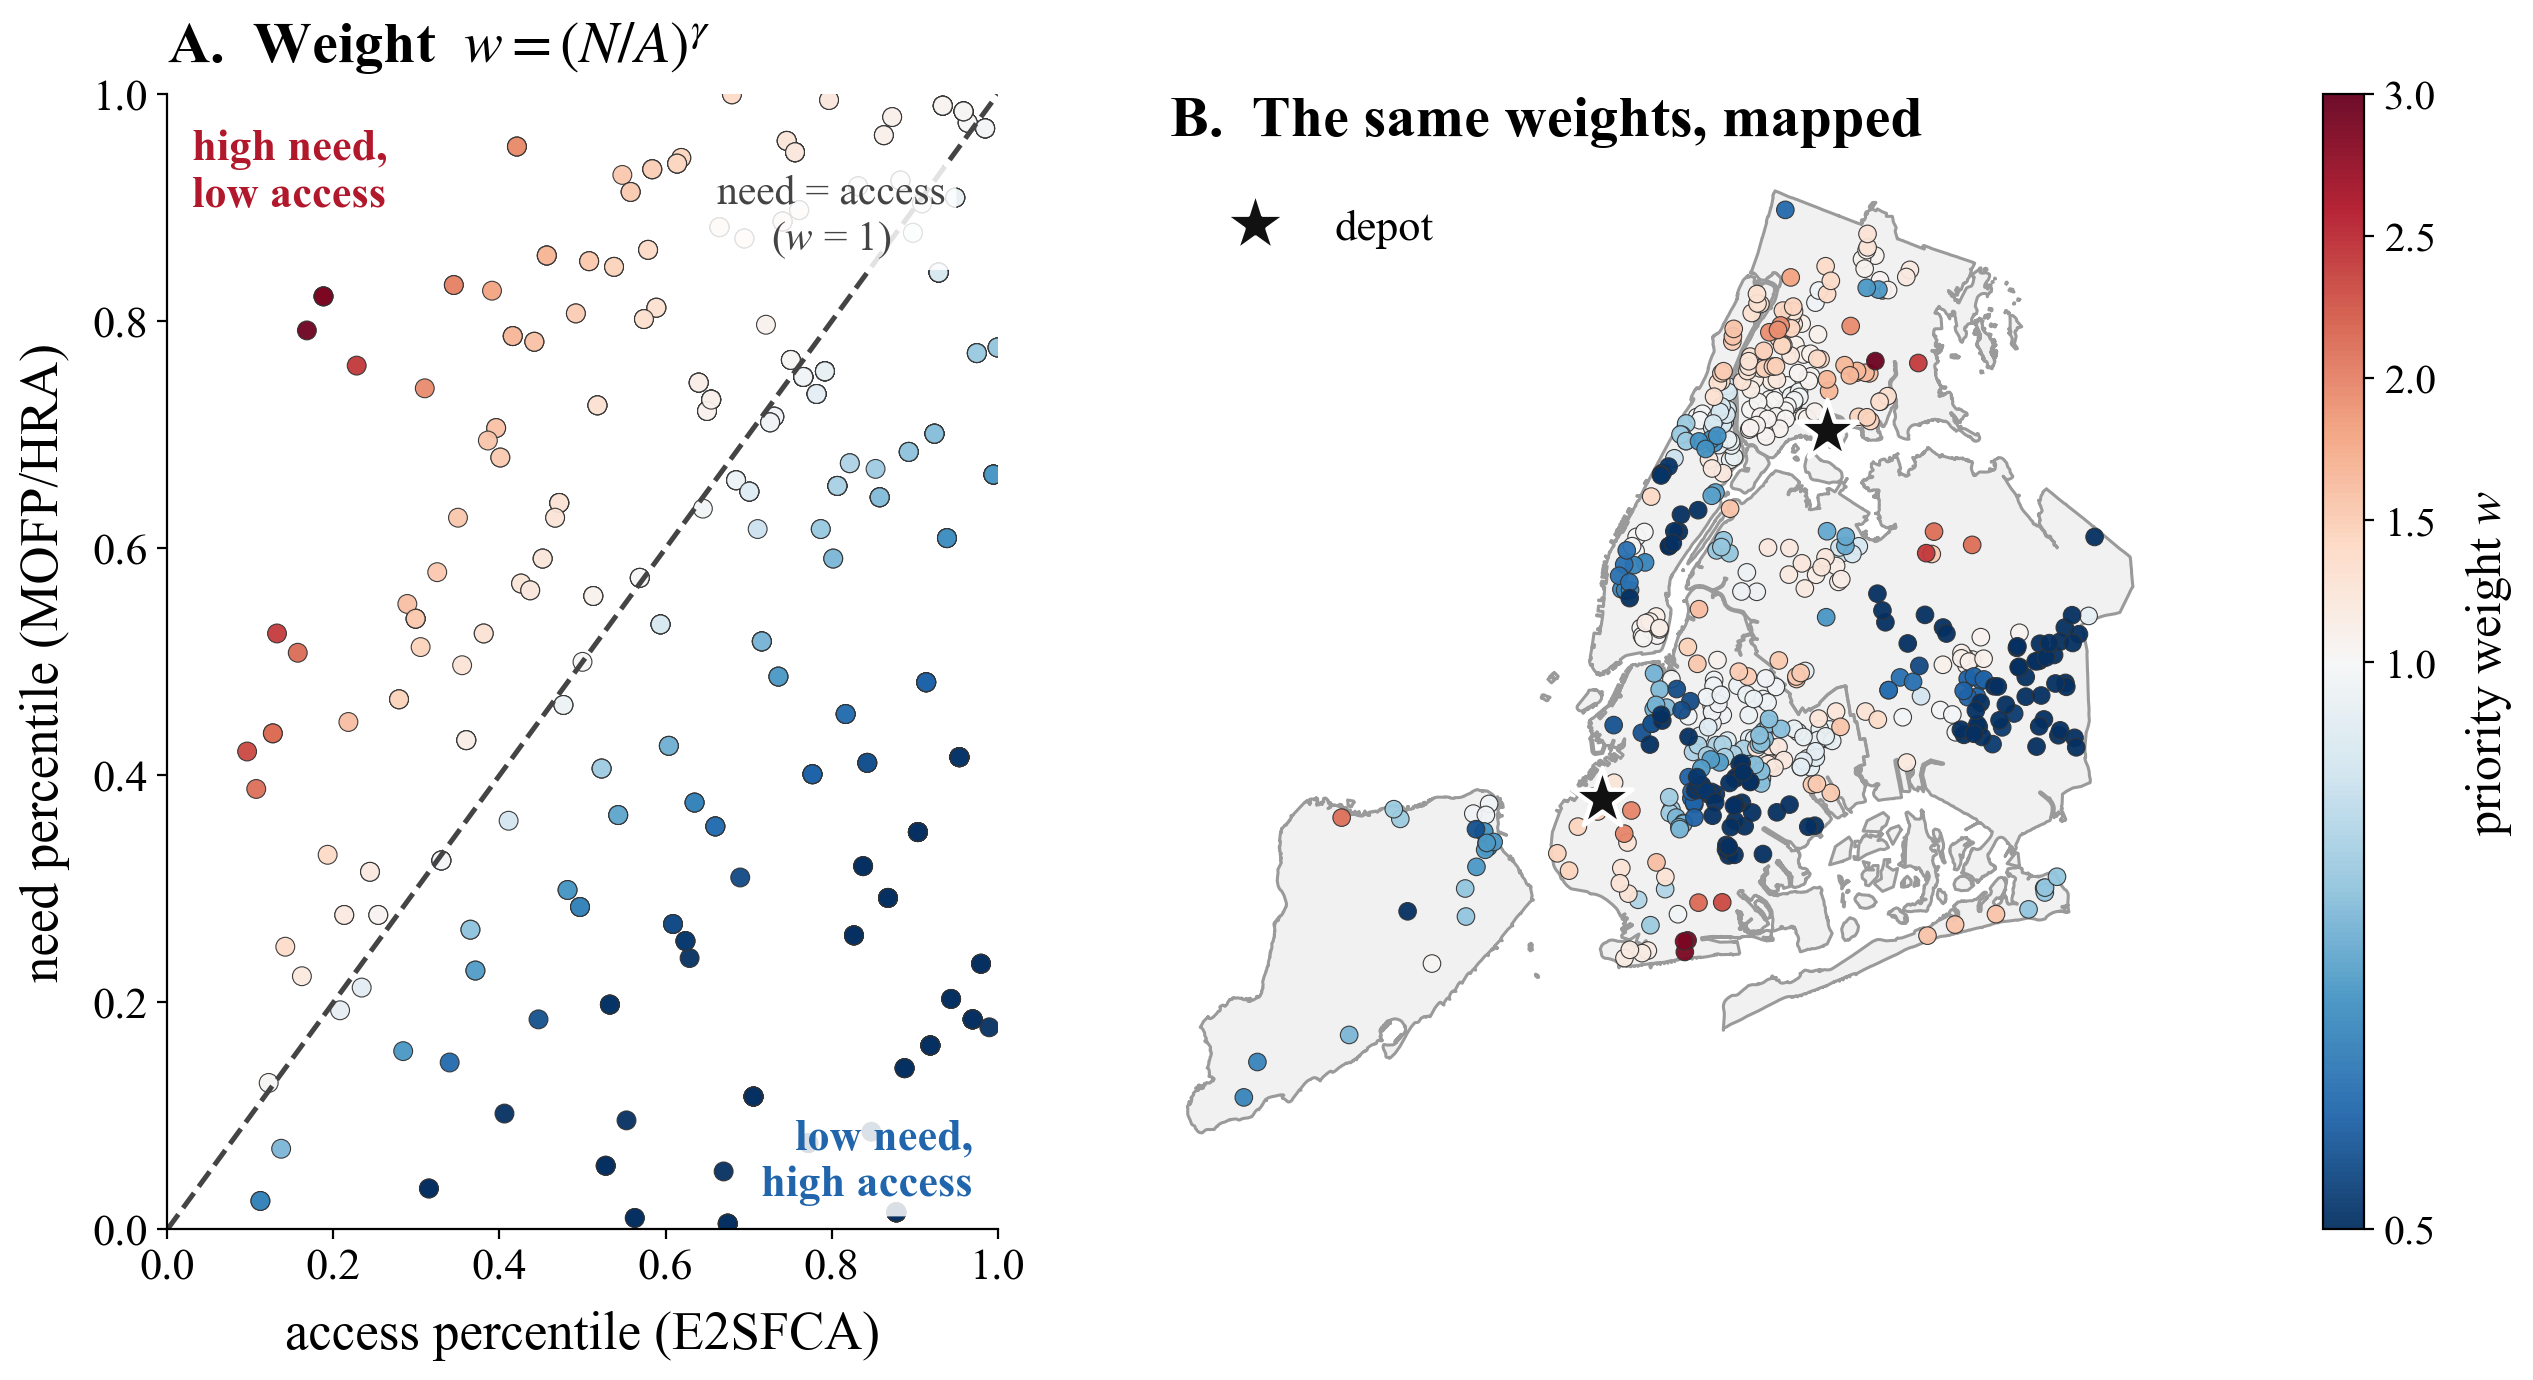
\includegraphics[width=0.88\linewidth]{figures/fig_equity_layer_poster.png}
      \caption{Priority weights at $\gamma = 1$: by need and access percentile (A)
      and on the map (B).}
    \end{figure}

  \end{block}

\end{column}

\separatorcolumn

% ============================================================ COLUMN 2
\begin{column}{\colwidth}

  \begin{block}{The Model}

    An optional-service pickup-and-delivery VRPTW. Binary $y_i$ marks whether
    recipient $i \in V$ is served, and $x_{ijk}$ whether vehicle $k \in K$ drives
    from $i$ to $j$. Each recipient's priority weight is

    \vspace{-0.7em}
    \begin{equation*}
      w_i \;=\; \mathrm{clip}\!\left(
        \left(\frac{N_i+\varepsilon}{A_i+\varepsilon}\right)^{\!\gamma},
        \; w_{\min},\, w_{\max}\right),
    \end{equation*}

    where $\varepsilon$ stabilizes the ratio near zero access. The exponent
    $\gamma$ is an \textbf{equity dial}: at $\gamma = 0$ every recipient counts equally; larger $\gamma$ favors underserved areas. The solver maximizes

    \vspace{-0.5em}
    \begin{equation*}
      \sum_{i \in V} P\, w_i\, y_i
      \;-\; \lambda \sum_{k \in K} \sum_{(i,j)} c_{ij}\, x_{ijk}
      \;-\; \delta \sum_{i \in V} \mathrm{cold}_i\, \tau_i ,
    \end{equation*}

    where $P$ is the base value of serving a recipient, $c_{ij}$ the travel time
    from $i$ to $j$, $\mathrm{cold}_i$ the refrigerated pounds due at $i$, and
    $\tau_i$ the arrival time there; $\lambda$ and $\delta$ set how heavily travel
    and late cold food count, subject to capacity, refrigeration, and time
    windows. Because $y_i$
    is a decision rather than a requirement, the model must choose whom to serve.
    \textbf{This is when the allocation comes in.}

    \textbf{Example instance:} 528 public recipient locations [4], 18 donors,
    25 vehicles, 2 depots, and OSRM road travel times. Fleet and demand
    parameters are labeled scenario assumptions.

    \textbf{Solution method:} routes are optimized with Google OR-Tools using
    guided local search, under a 30-second time budget per solve. Because a single
    solve varies by a few points, each strategy is solved five times with small random perturbations and reported by its median.

  \end{block}

\vspace{0.5em}

  \begin{block}{Strategies Compared}

    Every strategy faces the same 25 trucks, the same donated food, and the same opening
    hours, so any difference in who gets served traces back to the objective function alone.

    \begin{table}
      \centering
      \normalsize
      \begin{tabular*}{\linewidth}{@{\extracolsep{\fill}}lll@{}}
        \toprule
        \textbf{Strategy} & \textbf{Priority weight} & \textbf{Equity signal} \\
        \midrule
        Unweighted        & $1$ \;($\gamma = 0$)            & none \\
        Random-preference & $\mathcal{U}(0.3,\,1.7)$        & arbitrary \\
        Need-only         & need term only                  & need \\
        Access-only       & access term only                & access \\
        Need-access       & $(N_i/A_i)^{\gamma}$, $\gamma = 1$ & need $\div$ access \\
        \bottomrule
      \end{tabular*}
    \end{table}

  \end{block}

\vspace{0.2em}

  \begin{block}{Results Across Strategies}

    \begin{table}
      \vspace{-0.4em}
      \centering
      \normalsize
      \captionsetup{justification=centering, singlelinecheck=true}
      \caption{Medians of five replicate solves, need-access at $\gamma = 1$;
      highlights exceed replicate noise.}
      \begin{tabular*}{\linewidth}{@{\extracolsep{\fill}}lrrrrr@{}}
        \toprule
        \textbf{Metric} & \textbf{Unwt.} & \textbf{Random} & \textbf{Need}
          & \textbf{Access} & \textbf{Need-acc.} \\
        \midrule
        Sites served
          & 231 & 234 & 209 & 194 & 183 \\
        High-need tier \%
          & 26 & 25 & \textcolor{DodgerBlue}{\textbf{58}} & 22 & 44 \\
        Need-weighted \%$^\dagger$
          & 29 & 31 & 36 & 42 & \textcolor{DodgerBlue}{\textbf{46}} \\
        Travel (veh-min)
          & 12,412 & 13,034 & 12,991 & 13,501 & 13,146 \\
        \bottomrule
      \end{tabular*}

      \vspace{0.3em}
      {\small $^\dagger$Weights each recipient by $w$ at $\gamma = 1$: the ratio
      need-access maximizes.}
    \end{table}

    \textbf{Without an equity signal, service ignores need.} Unweighted and Random
    serve the most sites, yet reach only 26\% and 25\% of the \emph{high-need
    tier}: demand served among recipients in the neediest third of
    neighborhoods, a measure built from neighborhood need alone.

    \textbf{The yardstick picks the winner.} Need-only reaches 58\% of that tier
    and still serves more sites than need-access does. Need-access leads only on
    need-weighted coverage, which scores each recipient by the very ratio it
    optimizes. By that same measure Access-only ranks second, at 42\%, while doing
    no better than the two no-signal plans do on the high-need tier.

    \textbf{Travel barely moves.} Median fleet time differs by at most 9\% across all five strategies, comparable to the 7 to 14\% that a single strategy varies between its replicate solves.

  \end{block}

\end{column}

\separatorcolumn

% ============================================================ COLUMN 3
\begin{column}{\colwidth}

  \begin{block}{The Equity Dial}

    \begin{figure}
      \centering
      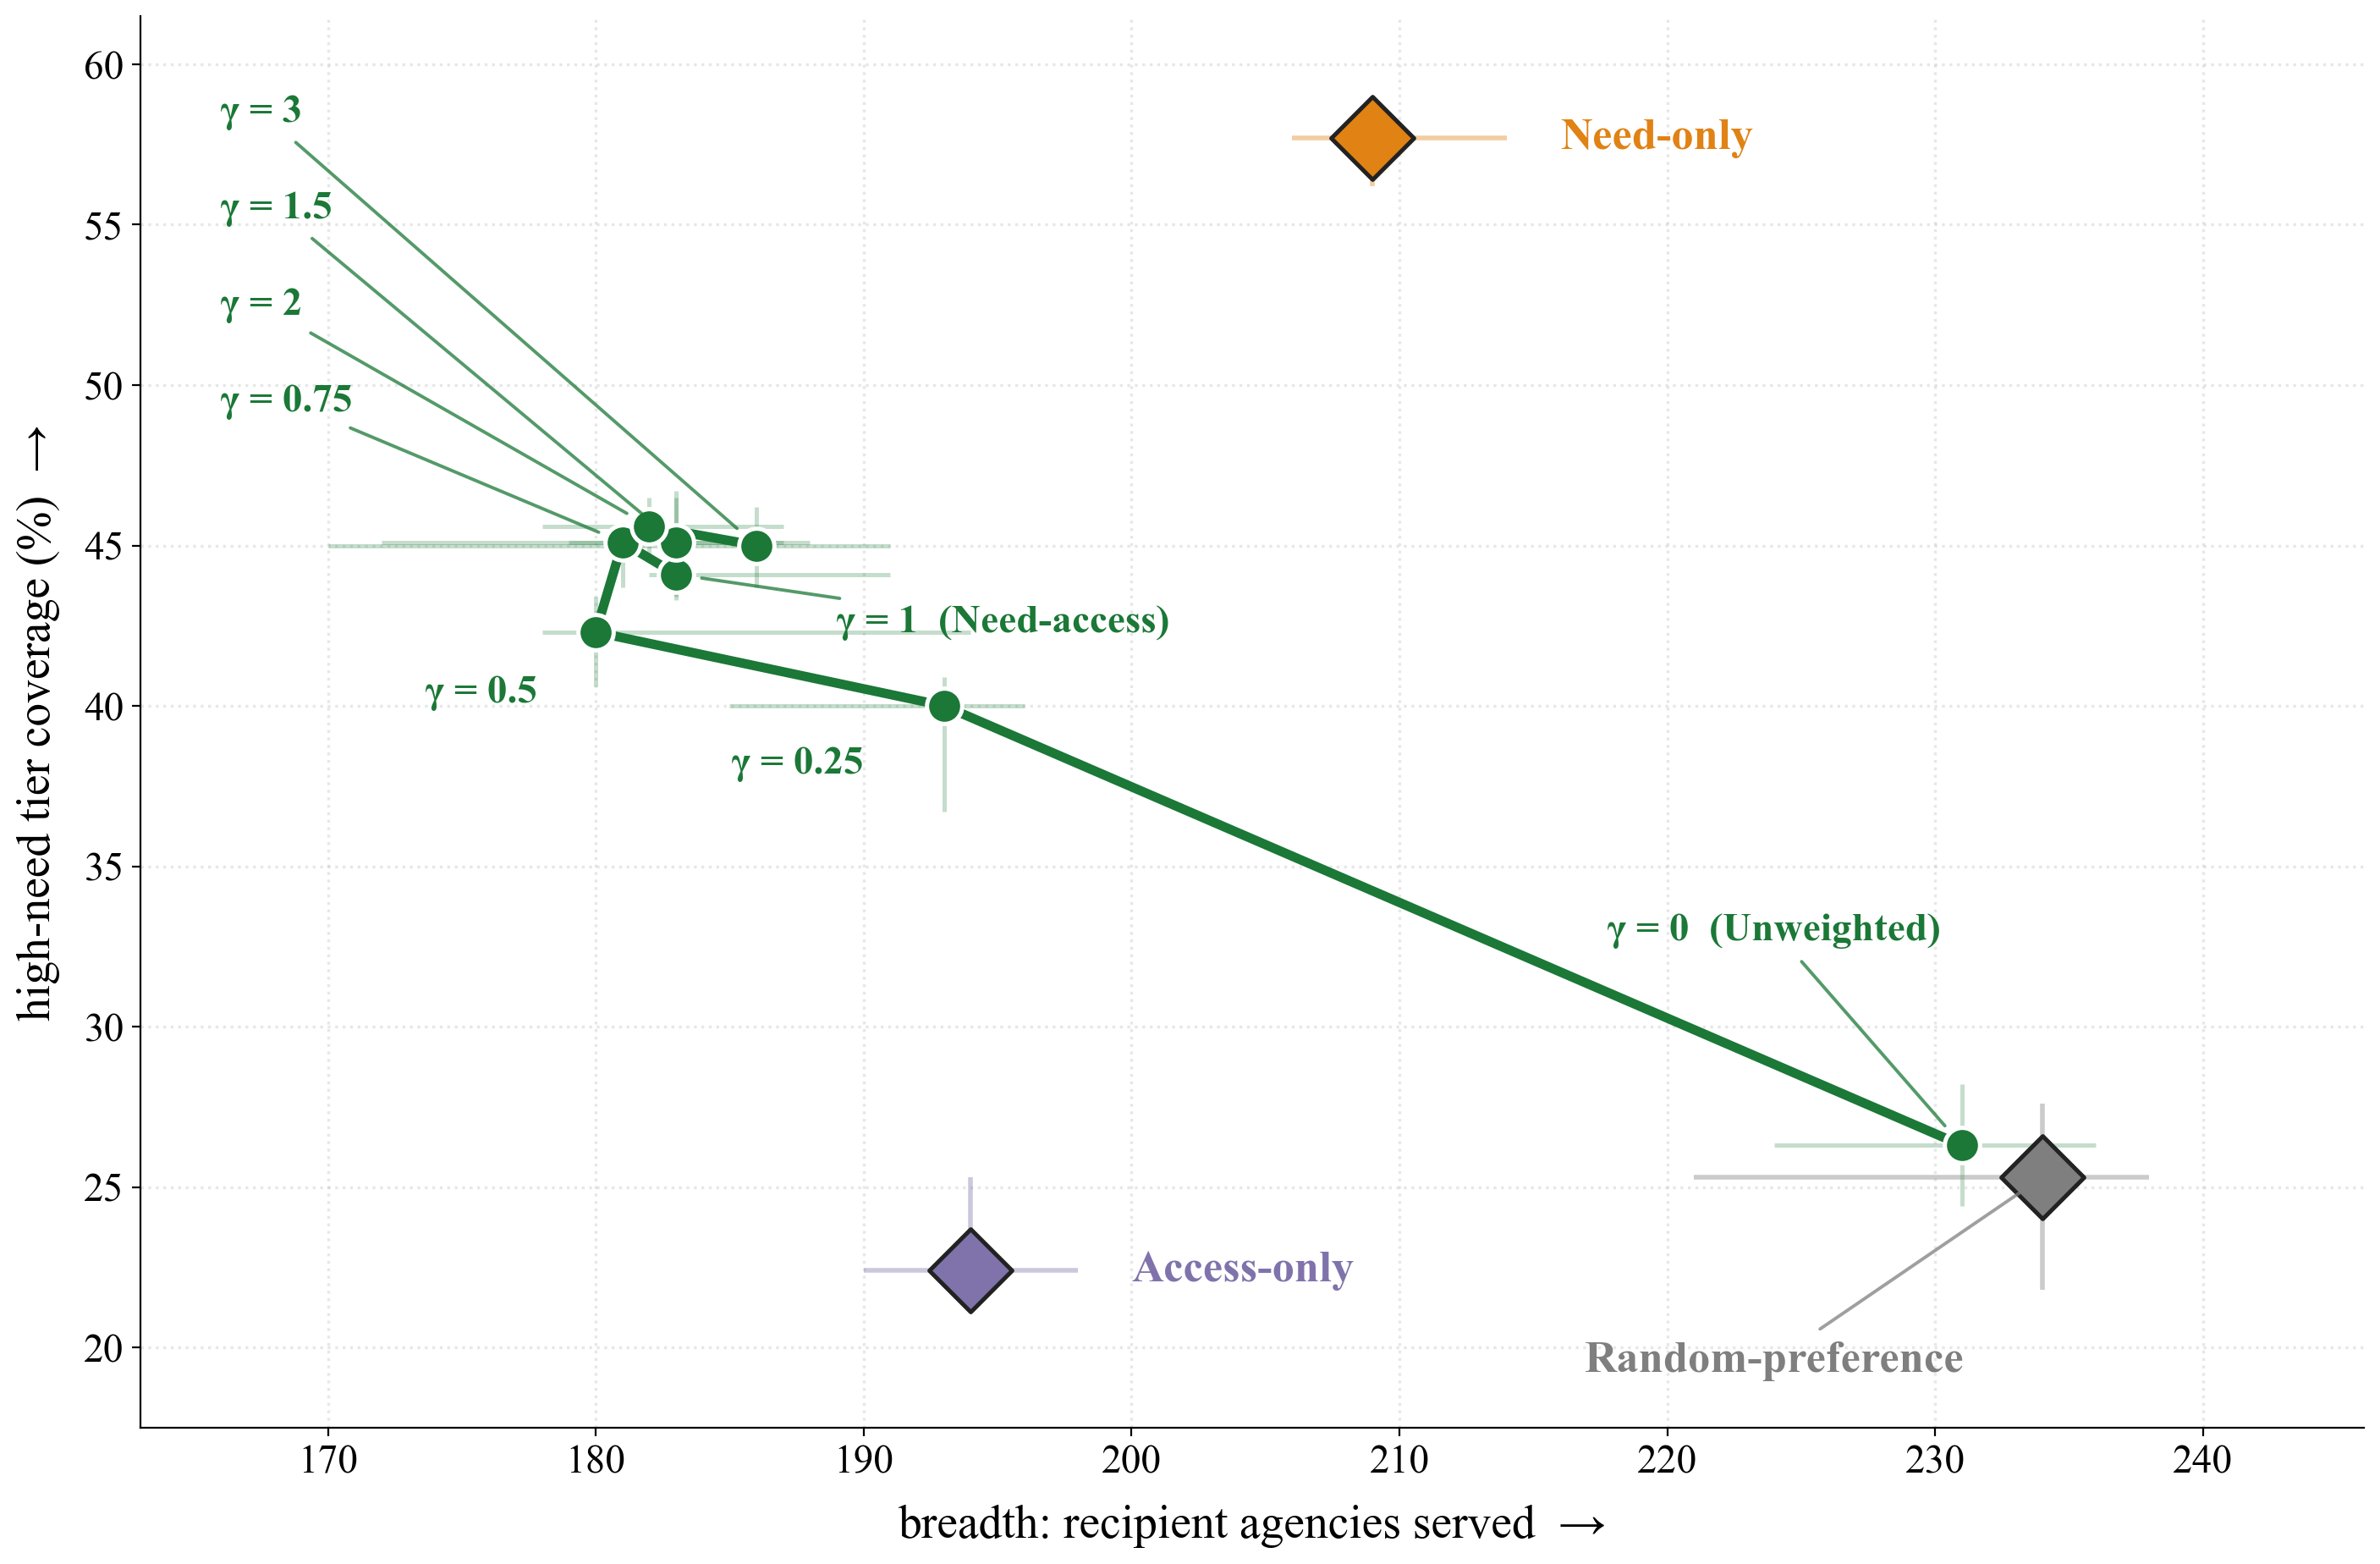
\includegraphics[width=0.92\linewidth]{figures/fig_dial_poster.png}
      \caption{Every strategy on two axes no objective optimizes directly. Points
      are medians of five replicate solves; whiskers show the range. The green
      curve is need-access as $\gamma$ rises; its $\gamma = 0$ end is Unweighted.}
    \end{figure}

    Most of the gain, and most of the cost, arrive in the first step:
    $\gamma = 0.25$ lifts high-need coverage from 26\% to 40\% and cuts sites
    served from 231 to 193. Past $\gamma \approx 0.75$ both plateau, near 45\% and
    183 sites, and the remaining wiggles sit inside replicate noise.
    \textbf{Need-only lies above and to the right of the entire curve}; even its
    worst replicate beats the curve's best on both axes. No setting of the dial reaches it; folding in access dilutes the model's focus on need.

  \end{block}

\vspace{0.8em}

  \begin{block}{Conclusion and Broader Impact}

    \begin{itemize}
      \item \textbf{Routing objectives are allocation policies.} Under scarcity
            every plan leaves someone unserved; without an equity signal, the choice falls to travel cost or to chance.
      \item \textbf{A fairness metric can grade itself.} Scored by its own
            weights, need-access looks like the best choice. Scored by need alone, need-only wins
            on both coverage and breadth, by margins wider than replicate noise, so the choice of yardstick is itself a policy decision.
      \item \textbf{Equity costs breadth, not driving.} Need-access served about a fifth fewer sites than Unweighted (183 versus 231), while total fleet time stayed within replicate noise.
    \end{itemize}

    This is decision-support evidence, not an operational recommendation: need is
    measured by neighborhood, access by provider hours, and the model plans a
    single representative day. Recipient-capacity uncertainty and delivery recourse are the next step to evaluate.

    \textbf{Broader impact.} Nonprofit staff described operational capacity, not only food supply, as what
    often limits how many people they reach. Allocation is therefore a lever
    that requires no additional trucks: the same fleet can be directed toward the
    neighborhoods that need it most, with no measurable change in driving. The
    framework also makes an otherwise invisible choice auditable, showing
    planners before dispatch which communities a plan leaves out. The same logic
    applies wherever demand exceeds capacity, from disaster relief to mobile
    health clinics and emergency supply delivery, wherever a fixed fleet must decide whom to reach first.

  \end{block}

\vspace{0.8em}

  \begin{block}{References}

    \small
    [1] Robin Hood \& Columbia Center on Poverty and Social Policy, \textit{Poverty
    Tracker Annual Report}, Vol.~8, 2026.\newline
    [2] NYC Council Data Team, ``Emergency Food in NYC''; NYC MOFP/HRA
    neighborhood prioritization data, 2026.\newline
    [3] Luo \& Qi, \textit{Health \& Place} 15(4), 2009.\newline
    [4] NYC HRA, Food Help NYC locations, 2026.\newline
    [5] Solomon, \textit{Operations Research} 35(2), 1987.\newline
    [6] Eisenhandler \& Tzur, \textit{Operations Research} 67(1), 2019.\newline
    [7] Orgut, Ivy, Uzsoy \& Wilson, \textit{IIE Transactions} 48(3), 2016.

  \end{block}

\end{column}

\separatorcolumn
\end{columns}
\end{frame}
\end{document}
